\chapter{Topology in quantum mechanics}
\label{sec:no_flat}
\subsection*{Particle moving around a Flux tube}
    
        
        To start off we are goin to talk about a very specific case of a quantum particle in a ring around a infinitely long solenoid.\\
        The hamiltonian of a particle with charge $-e$ moving through a magnetic field $\mathbf B= \nabla \times \mathbf A$ is
        \begin{equation} \label{EMHamiltonian}
                H=\frac 1{2m}(\mathbf p + e\mathbf A)^2 
        \end{equation}
        \begin{wrapfigure}{r}{.4\textwidth}
            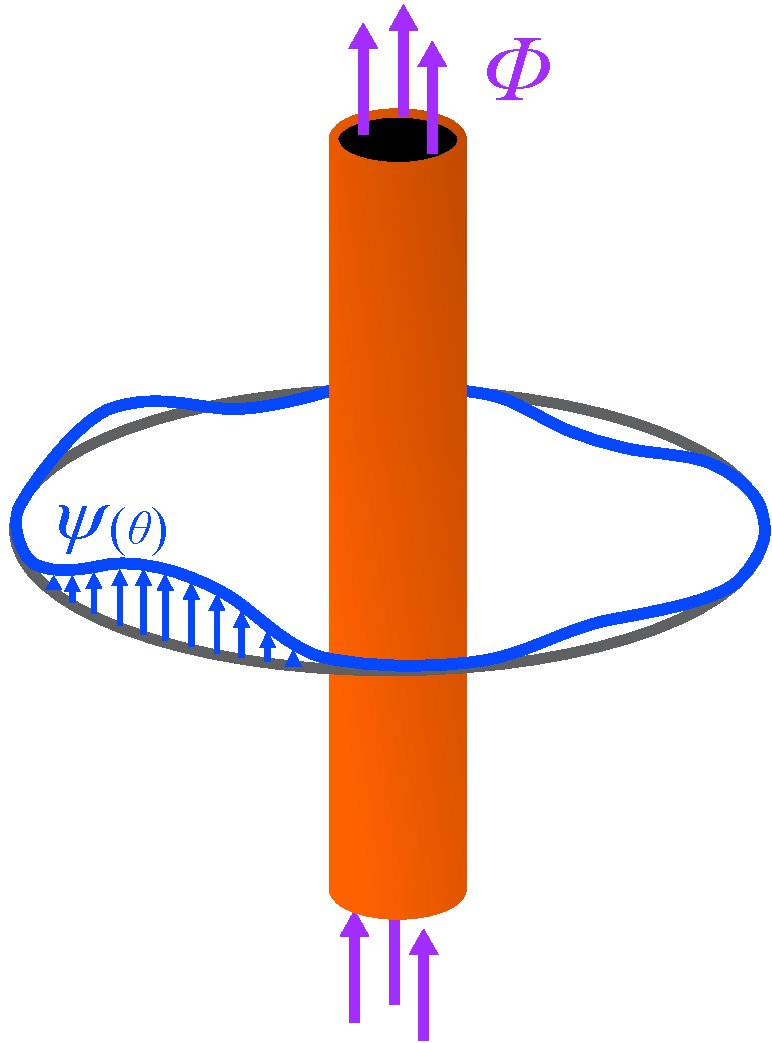
\includegraphics[width=.4\textwidth]{Immagini/topo/solenoid.pdf}
        \end{wrapfigure} 
        Since 
        \[\mathbf p=p_\theta \hat\theta=-\frac{i\hbar\mathbf {\hat \theta}}{R}\frac\partial {\partial \theta}\]
        \[
            \oint \mathbf A\cdot d\mathbf r=\int \mathbf B\cdot d\mathbf s = \Phi
        \]   
        it means that
        \begin{equation} \label{vector_potential}
            \mathbf A=\frac \Phi{2\pi R} \mathbf {\hat \theta}
        \end{equation}
        Putting it back into the hamiltonian
        \begin{equation} \label{EMHamiltonian2}
            H=\frac 1{2m}\bigg(-\frac{i\hbar}{R}\frac\partial {\partial \theta} + \frac{e\Phi}{2\pi R}\bigg)^2 
        \end{equation}
        The eigenstates of this hamiltonian are 
        \[
        \psi_n(\theta)=\frac {e^{in\theta}} {\sqrt{2\pi R}}; \quad n\in \mathbb Z
        \]
        Interestingly the Energies of the eigenstates are influenced by the vector potential
        \begin{equation} \label{spectral_flow}
                E_n=\frac 1{2mR^2}\bigg(\hbar n+ \frac{e\Phi}{2\pi}\bigg)^2=\tilde E\bigg(n+\frac{\Phi}{\Phi_0}\bigg)^2
        \end{equation}
        where
        \[
        \tilde E=\frac{\hbar^2}{2mR^2} \quad \textrm{and} \quad \Phi_0=\frac{2\pi \hbar}e
        \]
        Suppose now that we start with the turned soleind off, and place the particle in the $n=0$ ground
        state. If we increase the flux then, by the time we have reached $\Phi=\Phi_0$ , the $n=0$ state
        has transformed into the state that we previously labelled $n = 1$. Similarly, each state
        $n$ is shifted to the next state, $n + 1$ \footnote{It is tempting to invoke the adiabatic theorem
        here but, because of level crossing at $\Phi=\Phi_0/2$ it is not valid}.\\
        \begin{minipage}{\textwidth}
                    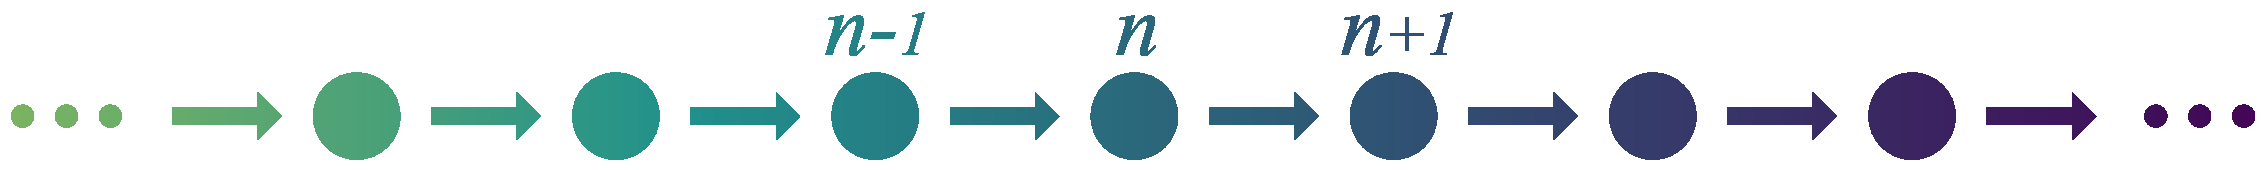
\includegraphics[width=1\linewidth]{Immagini/topo/flow.pdf}
        \end{minipage}
        This is an example of a phenomenon is called spectral flow: under a change of parameter
        the spectrum of the Hamiltonian changes, or “flows”. As we change increase the flux
        by one unit  $\Phi_0$ the spectrum returns to itself, but individual states have morphed into
        each other. \cite{tong2016lectures}
        \begin{figure}[h]
            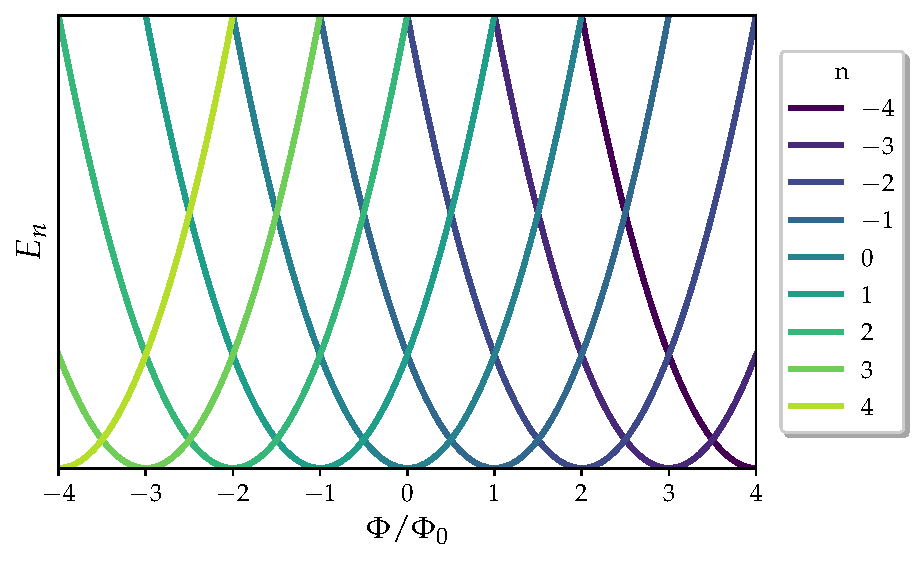
\includegraphics[width=\linewidth]{Immagini/topo/spectral_flow.pdf}
            \caption{Here plotted the energies $E_n$ (eq. \ref{spectral_flow} ), notice how the state \textit{"flow"} as we change $\Phi$}
        \end{figure}
    \subsection*{Parallelism with Bloch's Theorem}
    
        The keen eyed among you might have noticed that Figure 3 is suspicially similar to a crystal band structure in the limit on which the periodic potential $V\to 0$ with periodicity $2\pi$, let's see if this analogy holds \textit{the test of math}. Let's start by taking the single-particle free propagating Hamiltonian 
        \[
            H=\frac 1{2m}p_\theta^2
        \]
        The eigenstates this time have to respect the condition that $u_{n,q}(\theta)=e^{i2\pi q}u_{n,q}(\theta+2\pi)$.\footnote{This come from the block's theorem that states that the eigenstates of the hamiltonian of a periodic potential with periodicity $a$ mush obey that $u_{n,q}(x)=e^{iaq}u_{n,q}(x+a)$. In our case the periodicity $a=2\pi$ and the variable of the function is $\theta$ instead of $x$} This also means that if we substitute $q\to q+1$ the spectrum doesn't change. 
        % \begin{addmargin}[2em]{2em}
        %     \subsubsection*{Brief proof}
        %     A brief proof of this is the following:\\
        %     The problem of the eigenvalues can be written like so 
        %     \[
        %         He^{iq\theta}u_{n,q}(\theta)=E_n(q)e^{iq\theta}u_{n,q}(\theta)
        %     \]
        %     if we now send $q\to q+1$ the equation above becomes
        %     \[
        %         He^{iq\theta}e^{i\theta}u_{n,q+1}(\theta)=E_n(q+1)e^{iq\theta}e^{i\theta}u_{n,q+1}(\theta)
        %     \]
        %     The terms $u'_{n,q}(\theta)\equiv e^{i\theta}u_{n,q+1}(\theta)$ are also periodic $u'_{n,q}(\theta)=u'_{n,q}(\theta+2\pi)$. If we put it back into the equation above we get
        %     \[
        %         He^{iq\theta}u'_{n,q}(\theta)=E_n(q+1)e^{iq\theta}u'_{n,q}(\theta)
        %     \]
        %     That is completely equivalent to the equation at the start of this footnote, this means that the eigenvalues are periodic with periodicity 1\\
        % \end{addmargin}

        We now make the following unitary transformation to obtain a $q$-depentant Hamiltonian.
        \[
            H(q)=e^{-iq\theta}He^{iq\theta}=\frac 1{2m}\bigg (p_\theta + \frac {\hbar q}R \bigg)^2
        \]
        We can easly map this hamiltonian to the one in equation \ref{EMHamiltonian2} just by difining $\Phi$ such that $\hbar q= \frac {e\Phi}{2\pi}$. 
        \begin{equation} \label{blochA}
            H(\Phi)=\frac 1{2m}\bigg(p_\theta + \frac{e\Phi}{2\pi R}\bigg)^2
        \end{equation}
        Since before we said that the system doesn't change if we substitute $q\to q+1$, it means that now the system remains unchanged if we send $\Phi \to \Phi+\Phi_0$. This is exactly the result obtained in the previous page.
    
    
        And the tranformed eigenstates $\psi_{n,q}=e^{-iq\theta}u_{n,q}$ is just the cell-periodic part of the Bloch function. It satified the stricter periodic boundary condition
        \begin{equation} \label{blochboundraty}
            \psi_{n,q}(\theta)=\psi_{n,q}(\theta +2\pi)
        \end{equation}
        As you can see equations \ref{blochA}  and \ref{blochboundraty} create a system that is mathematically equivalent to the particle moving in a ring around a flux tube \cite{WeinbergBloch}.






    \subsection*{Conditions to have spectral flow}
        Up until now we looked spectral flow the case where the particle is freely propagating, let's see what happens when we add a periodic potential $V(\theta)=V(\theta+2\pi)$
        \[
            H=\frac 1{2m}p_\theta^2 + V(\theta)
        \]
        Now the spectrum is still periodic, however the energy bands don't necessarely cross, this means that  when abiabatically changing $q$, (or equivalently $\Phi$) the states won't flow, instead they will return to their original state
        \begin{figure}[h]
            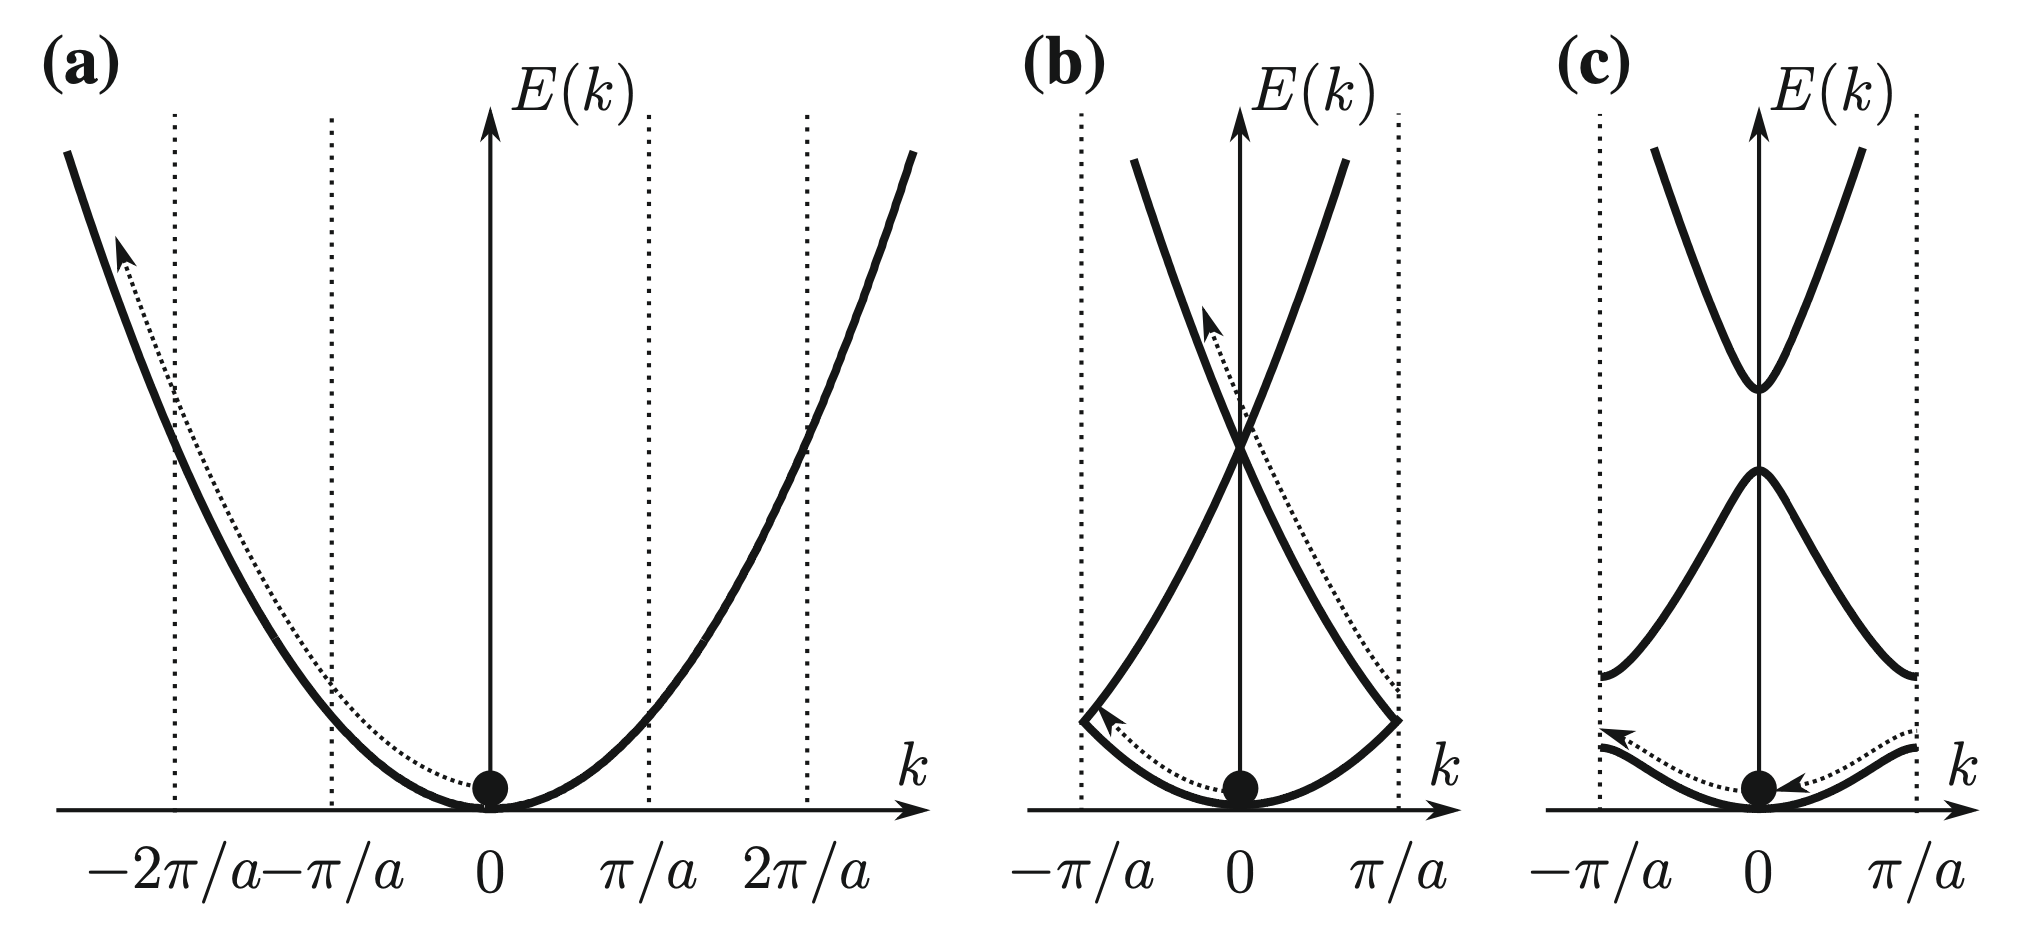
\includegraphics[width=\linewidth]{Immagini/topo/grosso-flow.png}
            \caption{Pictorial representation of what happens when changing $q$}
        \end{figure}
        Conversely if there are $n$ degeneracies, on every cycle more the $i$-th stathe will flow to the $i+n$-th state


    
    \subsection*{Spectral flow in a more general context}
    
        The spectral flow is applicable in much more complex geometries than the one we have seen so far.\\
        Suppose that now the particle can moove in a 3D potential $V(\mathbf r)$, the Hamiltonian is
        \[
            H(\mathbf A)=\frac 1{2m}(\mathbf p + e\mathbf A)^2 + V(\mathbf r) 
        \]

        Since the solenoid is still the same, the formula for $\mathbf A$ remains unchanged (eq. \ref{vector_potential} )
        \[
            H(\Phi)=\frac 1{2m}\bigg(\mathbf p + \frac{e\Phi}{2\pi R}\hat \theta\bigg)^2 + V(\mathbf r)
        \]
        and since it's expressed in cylindrical coordinates it's better to express also $\mathbf p$ in cylindrical coordinates.
        \[
         \mathbf p =-i\hbar \mathbf \nabla=-i\hbar\bigg( 
             \mathbf{\hat r}\frac{\partial}{\partial r}+ \frac{\mathbf {\hat \theta}}{r}\frac{\partial}{\partial \theta} + \mathbf{\hat z}\frac{\partial}{\partial z}  \bigg) \equiv
             \mathbf{\hat r} p_r+ \mathbf {\hat \theta} p_\theta + \mathbf{\hat z} p_z
        \]
        Of course if we send $\theta \to \theta + 2\pi$ the system should be unchanged.
        \[
            \psi(r,\theta,z)=\psi(r,\theta+2\pi,z)
        \]
        Following the inverse reasoning done in the previous subsection we make the following unitary transformation.
        \[
            H=e^{i\theta\Phi/\Phi_0}H(\Phi)e^{-i\theta\Phi/\Phi_0}=\frac  {\mathbf p^2} {2m} + V(\mathbf r)
        \]
        This means that the eigenvalue probelm is now written like so
        \[
            He^{i\theta\Phi/\Phi_0}\psi(r,\theta,z)=E(\Phi)e^{i\theta\Phi/\Phi_0}\psi(r,\theta,z)
        \]

        If we send $\Phi \to \Phi+\Phi_0$ we get an equivalent equation
        \[
            He^{i\theta\Phi/\Phi_0}\psi(r,\theta,z)=E(\Phi+\Phi_0)e^{i\theta\Phi/\Phi_0}\psi(r,\theta,z)
        \]

        this means that the energy spectrum is unchanged if we send $\Phi \to \Phi+\Phi_0$. This is true regardless of the shape or geometry of $V(\mathbf r)$.
        
    
    \subsection*{The quantum Hall effect}

    
    
        We'll now see the effects of the spectral flow on physical properties of materials. Suppose we have a system like the one of the figure on the side. Now we slowly increase $\Phi$ from 0 to $\Phi_0$ in a total time $T$. This introduces a electromagnetice force arround the ring $\mathcal{E}=-\partial_t\Phi=-\Phi_0/T$.
    
    
        Let's suppose that the disc has the property that due to spectral flow $n$ electrons are transferred form the inner cirlce to the outer cicle in this time $T$. This would result in a radial current $I_r=-ne/T$. This means that the resistance is 
        \begin{equation} 
            \label{hall_resistivity}
                R_{xy}=\frac{\mathcal {E}}{I_r}=\frac{2\pi\hbar}{e^2}\frac 1n
        \end{equation}
        However, to be able to calculate $n$ we need to calculate how is the spectrum of the system as we change $\Phi$. This means that $n$ depends on the system, but equation \ref{hall_resistivity} is independent of the system. \footnote{There is the caveaut here that the system has to be in a defined quantum state, so in real world system it means that $T\approx0$}